% =============================================================================
% Chapter 5 — Testing and Evaluation
% =============================================================================
\chapter{Testing and Evaluation}
\label{ch:testing-evaluation}

This chapter presents the systematic evaluation of the ADHD Second Brain application across all five project objectives. Each subsystem is evaluated independently before assessing end-to-end pipeline performance. The chapter concludes with a reproducibility assessment and a traceability matrix mapping evaluation results to the project objectives defined in \cref{sec:objectives}.

% -----------------------------------------------------------------------------
\section{Testing Strategy and Methodology}
\label{sec:testing-strategy}

The evaluation framework comprises over 220 automated tests distributed across 25 test files, executed through the pytest framework. Tests span four levels of granularity: unit tests validating individual functions in isolation, integration tests verifying inter-module communication, end-to-end pipeline tests exercising the complete inference chain, and benchmark tests measuring quantitative performance metrics under controlled conditions. A dedicated SetFit wiring verification suite (20~tests) validates the end-to-end integration between emotion classification, PASE radar mapping, confidence gating, and JITAI intervention triggering. Five synthetic ADHD personas---covering the full spectrum of six emotion categories and diverse screen activity patterns---were used to exercise the system across representative emotional states and task contexts.

All benchmarks were executed on a MacBook Pro with the Apple M4 system-on-chip, 16~GB of unified memory, and macOS~15 Sequoia. A two-run protocol with a fixed random seed of 42 was adopted for all stochastic benchmarks, with consolidated results computed as the arithmetic mean and the coefficient of variation (CV) reported for each metric. Energy measurements were collected using \texttt{zeus-apple-silicon}, reading Apple Silicon power telemetry registers at 100~ms intervals with idle power subtracted.

% -----------------------------------------------------------------------------
\section{Emotion Classification Evaluation}
\label{sec:emotion-evaluation}

This section evaluates three classification approaches---a hybrid embedding-SenticNet pipeline, a SetFit contrastive learning pipeline, and a DistilBERT fine-tuning pipeline---across nine experimental configurations, documenting the progression from a 28\% baseline to the production model's 86\% accuracy.

\subsection{Baseline and Approach Comparison}
\label{subsec:baseline-comparison}

The baseline classifier mapped SenticNet sentiment polarity ranges to the six ADHD emotion categories through hand-crafted thresholds, achieving only 28\% accuracy (macro-F1 0.264)---barely above the 16.7\% random chance for six classes. \Cref{tab:classification-results} presents the complete results across all nine configurations. Three findings are key.

First, the hybrid approach (Approach~A) achieved 74\% accuracy with embeddings alone, but incorporating SenticNet features \emph{degraded} performance to 70\%. The Hourglass dimensions operate at a coarser semantic granularity than the six ADHD categories, introducing noise that diluted embedding discriminative power. This directly informed the decision to use SenticNet exclusively for coaching enrichment.

Second, the SetFit contrastive learning pipeline (Approach~B) achieved 86\% with only 210 training sentences. The optimisation from 80\% to 86\% involved four changes: replacing the default loss with CoSENTLoss \cite{reimers2019}, upgrading the encoder to \texttt{all-mpnet-base-v2}, switching to exhaustive all-unique-pairs generation, and incorporating hard negative mining. Prediction confidence increased from 0.33 to 0.76.

Third, augmenting the 210 sentences with 288 LLM-generated sentences (498 total) caused regression to 82\%. The anxious category F1 dropped from 0.80 to 0.62 due to class imbalance and boundary blurring, underscoring the need for curated rather than bulk data augmentation.

The DistilBERT approach (Approach~C) achieved 62\% with 210 samples and 72\% with 1,200 augmented samples. A HuggingFace pre-collected dataset of 30,000 samples produced only 32\% due to severe domain mismatch, demonstrating that dataset relevance dominates dataset size for domain-specific tasks.

\begin{table}[htbp]
  \centering
  \caption{Emotion classification results across all approaches and configurations.}
  \label{tab:classification-results}
  \begin{tabular}{@{}llcccc@{}}
    \toprule
    & \textbf{Approach} & \textbf{Training Data} & \textbf{Accuracy} & \textbf{Macro-F1} & \textbf{Avg.\ Conf.} \\
    \midrule
    & Baseline (SenticNet only) & N/A & 28\% & 0.264 & --- \\
    A & Hybrid (embedding only) & 210 & 74\% & 0.732 & --- \\
    A & Hybrid (+ SenticNet) & 210 & 70\% & 0.688 & --- \\
    B & SetFit (initial) & 210 & 80\% & 0.803 & 0.33 \\
    B & \textbf{SetFit (optimised)} & \textbf{210} & \textbf{86\%} & \textbf{0.862} & \textbf{0.76} \\
    B & SetFit (expanded) & 498 & 82\% & 0.819 & --- \\
    C & DistilBERT (10 epoch) & 210 & 62\% & 0.568 & --- \\
    C & DistilBERT (augmented) & 1,200 & 72\% & 0.727 & --- \\
    C & DistilBERT (HuggingFace) & 30,000 & 32\% & 0.265 & --- \\
    \bottomrule
  \end{tabular}
\end{table}

\subsection{SetFit Optimisation Analysis}
\label{subsec:setfit-optimisation}

The progression from 80\% to 86\% was achieved through systematic ablation of four components. CoSENTLoss was the most impactful change, producing smoother gradient signals than the default triplet loss. The encoder upgrade from \texttt{all-MiniLM-L6-v2} (22M parameters, 384-d) to \texttt{all-mpnet-base-v2} (109M parameters, 768-d) provided richer representations. Exhaustive pair generation maximised information extracted from the 210-sentence corpus, and hard negative mining forced fine-grained distinctions between categories such as frustrated versus overwhelmed.

One training epoch consistently outperformed two (86\% vs 84\%), indicating susceptibility to overfitting. Learning rate sweeps produced no variation in one-epoch performance, suggesting robustness to optimiser configuration.

\subsection{Per-Class Performance}
\label{subsec:per-class-performance}

\Cref{tab:per-class-f1} presents per-class F1 scores for the production SetFit model on 50 held-out test sentences. Joyful achieved the highest F1 (0.89) due to distinctive lexical markers. Frustrated and overwhelmed achieved the lowest (0.74 each), reflecting genuine semantic overlap between these high-arousal negative states.

\begin{table}[htbp]
  \centering
  \caption{Per-class F1 scores for the production SetFit model.}
  \label{tab:per-class-f1}
  \begin{tabular}{@{}lcc@{}}
    \toprule
    \textbf{Category} & \textbf{F1 Score} & \textbf{Support} \\
    \midrule
    Joyful      & 0.89 & $\sim$8 \\
    Focused     & 0.80 & $\sim$8 \\
    Frustrated  & 0.74 & $\sim$8 \\
    Anxious     & 0.80 & $\sim$8 \\
    Disengaged  & 0.86 & $\sim$8 \\
    Overwhelmed & 0.74 & $\sim$9 \\
    \midrule
    Macro Average & 0.862 & 50 \\
    \bottomrule
  \end{tabular}
\end{table}

\subsection{Confusion Matrix Analysis}
\label{subsec:confusion-matrix}

\Cref{fig:confusion-matrix} presents the confusion matrix for the production SetFit model. Two primary confusion patterns emerge: a frustrated--overwhelmed axis (clinically expected, as the boundary between anger-driven task difficulty and cognitive overload is ambiguous even for human annotators) and a focused--anxious axis (high-attention language can resemble anxious hyper-vigilance). The diagonal dominance---39 correct out of 50---confirms reliable discrimination across all six categories.

% --- MERMAID BACKUP ---
% ```mermaid
% graph LR
%   subgraph "Confusion Matrix (SetFit Production)"
%     A["Predicted vs Actual 6x6 heatmap"]
%     B["joyful:     7, 0, 0, 0, 1, 0"]
%     C["focused:    0, 7, 0, 1, 0, 0"]
%     D["frustrated: 0, 0, 6, 0, 1, 1"]
%     E["anxious:    0, 1, 0, 6, 0, 1"]
%     F["disengaged: 0, 0, 1, 0, 7, 0"]
%     G["overwhelmed:0, 0, 1, 1, 0, 6"]
%   end
% ```
% --- END MERMAID ---

\begin{figure}[htbp]
  \centering
  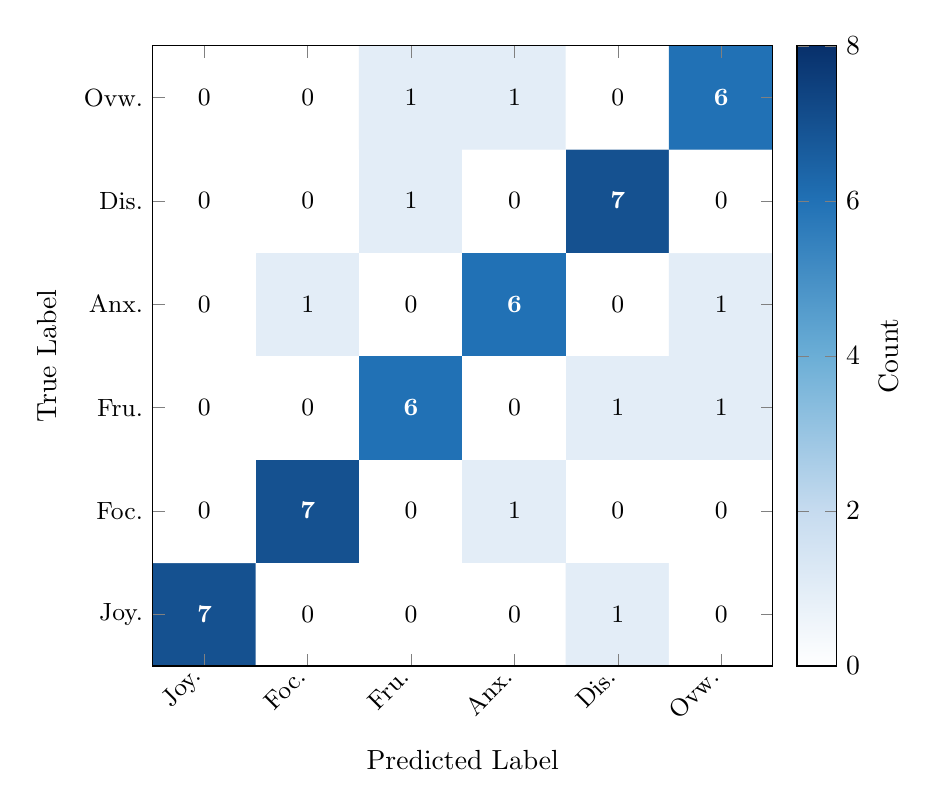
\begin{tikzpicture}
    \begin{axis}[
      width=0.78\textwidth,
      height=0.78\textwidth,
      enlargelimits=false,
      colormap={WhiteBlue}{
        rgb255(0cm)=(255,255,255)
        rgb255(1cm)=(198,219,239)
        rgb255(2cm)=(107,174,214)
        rgb255(3cm)=(33,113,181)
        rgb255(4cm)=(8,48,107)
      },
      colorbar,
      colorbar style={
        ylabel={Count},
        ytick={0,2,4,6,8},
      },
      point meta min=0,
      point meta max=8,
      xtick={0,1,2,3,4,5},
      ytick={0,1,2,3,4,5},
      xticklabels={Joy., Foc., Fru., Anx., Dis., Ovw.},
      yticklabels={Ovw., Dis., Anx., Fru., Foc., Joy.},
      x tick label style={font=\small, rotate=45, anchor=east},
      y tick label style={font=\small},
      xlabel={Predicted Label},
      ylabel={True Label},
      xlabel style={at={(0.5,-0.12)}},
      ylabel style={at={(-0.14,0.5)}},
      xmin=-0.5, xmax=5.5,
      ymin=-0.5, ymax=5.5,
    ]
      % Matrix data: rows from top (y=5 = joyful) to bottom (y=0 = overwhelmed)
      \addplot[
        matrix plot,
        point meta=explicit,
        mesh/cols=6,
        mesh/rows=6,
      ] coordinates {
        (0,5) [7]  (1,5) [0]  (2,5) [0]  (3,5) [0]  (4,5) [1]  (5,5) [0]
        (0,4) [0]  (1,4) [7]  (2,4) [0]  (3,4) [1]  (4,4) [0]  (5,4) [0]
        (0,3) [0]  (1,3) [0]  (2,3) [6]  (3,3) [0]  (4,3) [1]  (5,3) [1]
        (0,2) [0]  (1,2) [1]  (2,2) [0]  (3,2) [6]  (4,2) [0]  (5,2) [1]
        (0,1) [0]  (1,1) [0]  (2,1) [1]  (3,1) [0]  (4,1) [7]  (5,1) [0]
        (0,0) [0]  (1,0) [0]  (2,0) [1]  (3,0) [1]  (4,0) [0]  (5,0) [6]
      };

      % Cell annotations — joyful (y=5)
      \node[font=\small\bfseries, text=white] at (axis cs:0,5) {7};
      \node[font=\small] at (axis cs:1,5) {0};
      \node[font=\small] at (axis cs:2,5) {0};
      \node[font=\small] at (axis cs:3,5) {0};
      \node[font=\small] at (axis cs:4,5) {1};
      \node[font=\small] at (axis cs:5,5) {0};
      % focused (y=4)
      \node[font=\small] at (axis cs:0,4) {0};
      \node[font=\small\bfseries, text=white] at (axis cs:1,4) {7};
      \node[font=\small] at (axis cs:2,4) {0};
      \node[font=\small] at (axis cs:3,4) {1};
      \node[font=\small] at (axis cs:4,4) {0};
      \node[font=\small] at (axis cs:5,4) {0};
      % frustrated (y=3)
      \node[font=\small] at (axis cs:0,3) {0};
      \node[font=\small] at (axis cs:1,3) {0};
      \node[font=\small\bfseries, text=white] at (axis cs:2,3) {6};
      \node[font=\small] at (axis cs:3,3) {0};
      \node[font=\small] at (axis cs:4,3) {1};
      \node[font=\small] at (axis cs:5,3) {1};
      % anxious (y=2)
      \node[font=\small] at (axis cs:0,2) {0};
      \node[font=\small] at (axis cs:1,2) {1};
      \node[font=\small] at (axis cs:2,2) {0};
      \node[font=\small\bfseries, text=white] at (axis cs:3,2) {6};
      \node[font=\small] at (axis cs:4,2) {0};
      \node[font=\small] at (axis cs:5,2) {1};
      % disengaged (y=1)
      \node[font=\small] at (axis cs:0,1) {0};
      \node[font=\small] at (axis cs:1,1) {0};
      \node[font=\small] at (axis cs:2,1) {1};
      \node[font=\small] at (axis cs:3,1) {0};
      \node[font=\small\bfseries, text=white] at (axis cs:4,1) {7};
      \node[font=\small] at (axis cs:5,1) {0};
      % overwhelmed (y=0)
      \node[font=\small] at (axis cs:0,0) {0};
      \node[font=\small] at (axis cs:1,0) {0};
      \node[font=\small] at (axis cs:2,0) {1};
      \node[font=\small] at (axis cs:3,0) {1};
      \node[font=\small] at (axis cs:4,0) {0};
      \node[font=\small\bfseries, text=white] at (axis cs:5,0) {6};
    \end{axis}
  \end{tikzpicture}
  \caption{Confusion matrix for the production SetFit emotion classifier evaluated on 50 held-out test sentences. Diagonal entries indicate correct classifications; off-diagonal entries indicate misclassifications. The primary confusion axes lie between frustrated/overwhelmed and focused/anxious.}
  \label{fig:confusion-matrix}
\end{figure}

% -----------------------------------------------------------------------------
\section{LLM Performance Evaluation}
\label{sec:llm-evaluation}

\subsection{Throughput and Latency}
\label{subsec:llm-throughput}

\Cref{tab:llm-performance} presents inference performance for Qwen3-4B on the MLX framework. The overall throughput of 37.1 tokens per second exceeds the 30 tok/s target by 23.7\%, with a CV of only 0.8\% across runs. Throughput was stable across input lengths (short: 38.1, medium: 35.9, long: 37.3 tok/s). Cold start latency averaged 0.94~s with the highest variability (33.8\% CV) due to the initial transfer of 2.3~GB of quantised weights into GPU-accessible memory---this occurs only once per application launch.

The \texttt{/think} mode produced approximately 212 tokens in 4,738~ms, while \texttt{/no\_think} mode produced approximately 77 tokens in 2,046~ms. The application defaults to \texttt{/no\_think} for routine coaching, reserving \texttt{/think} for complex queries.

\begin{table}[htbp]
  \centering
  \caption{LLM inference performance metrics (consolidated across two runs, seed 42).}
  \label{tab:llm-performance}
  \begin{tabular}{@{}lcccc@{}}
    \toprule
    \textbf{Metric} & \textbf{Run 1} & \textbf{Run 2} & \textbf{Consolidated} & \textbf{CV} \\
    \midrule
    Throughput (short)       & 38.2 tok/s & 37.9 tok/s & 38.1 tok/s  & 0.6\% \\
    Throughput (medium)      & 35.4 tok/s & 36.4 tok/s & 35.9 tok/s  & 2.0\% \\
    Throughput (long)        & 37.2 tok/s & 37.4 tok/s & 37.3 tok/s  & 0.4\% \\
    Overall throughput       & ---        & ---        & 37.1 tok/s  & 0.8\% \\
    Cold start               & 0.80 s     & 1.07 s     & 0.94 s      & 33.8\% \\
    \texttt{/think} mode     & ---        & ---        & 4,738 ms ($\sim$212 tok) & --- \\
    \texttt{/no\_think} mode & ---        & ---        & 2,046 ms ($\sim$77 tok)  & --- \\
    \midrule
    RSS (with model)         & ---        & ---        & $\sim$2,854 MB & --- \\
    GPU memory               & ---        & ---        & $\sim$2.3 GB   & --- \\
    \bottomrule
  \end{tabular}
\end{table}

\subsection{Memory Footprint}
\label{subsec:llm-memory}

The RSS with the model loaded was approximately 2,854~MB, of which 2.3~GB was attributable to quantised model weights. This is well within the 6~GB target (Objective~5), leaving substantial headroom for the emotion classifier ($\sim$450~MB), Mem0 memory system ($\sim$502~MB), and typical knowledge worker applications on a 16~GB MacBook Pro \cite{hannun2023, lin2025, xu2024}.

% -----------------------------------------------------------------------------
\section{SenticNet Pipeline Evaluation}
\label{sec:senticnet-evaluation}

\subsection{Latency Scaling}
\label{subsec:senticnet-latency}

\Cref{tab:senticnet-latency} presents SenticNet pipeline latency by input length. Latency scales approximately linearly with word count, but per-word cost decreases from 260~ms (10 words) to 45~ms (200 words) as fixed overhead is amortised. For typical user messages (10--50 words), latency stays within 2,600--3,300~ms.

\begin{table}[htbp]
  \centering
  \caption{SenticNet pipeline latency by input length.}
  \label{tab:senticnet-latency}
  \begin{tabular}{@{}rcr@{}}
    \toprule
    \textbf{Input Length} & \textbf{Mean Latency} & \textbf{Per-Word Cost} \\
    \midrule
    10 words  & 2,600 ms & 260 ms/word \\
    50 words  & 3,300 ms & 62 ms/word  \\
    100 words & 4,500 ms & 48 ms/word  \\
    200 words & 9,100 ms & 45 ms/word  \\
    \bottomrule
  \end{tabular}
\end{table}

\subsection{Reliability and Determinism}
\label{subsec:senticnet-reliability}

The single SenticNet API call exhibited a median latency of 521~ms (CV 3\%) with 100\% reliability over 100 consecutive calls. The Hourglass of Emotions values were fully deterministic across runs---identical values for identical input concepts---simplifying testing and ensuring reproducible affective enrichment \cite{cambria2024, cambria2016}.

% -----------------------------------------------------------------------------
\section{SetFit Wiring Verification}
\label{sec:setfit-wiring-evaluation}

A dedicated test suite of 20~tests validates the end-to-end integration between the SetFit emotion classifier, the PASE radar mapping, the confidence-gated JITAI rules, and the dashboard pipeline. All 20~tests passed.

\subsection{Emotion Radar PASE Mapping}
\label{subsec:pase-tests}

Six tests verified the \texttt{blend\_pase} function: (1)~all six SetFit labels have valid PASE mappings with all four keys present; (2)~high confidence ($>$0.9) produces profiles within 0.05 of the canonical values; (3)~low confidence ($<$0.1) produces profiles within 0.1 of neutral (0.5); (4)~zero confidence produces exactly neutral profiles; (5)~all PASE values remain within $[0, 1]$ across all labels and confidence levels; and (6)~unknown labels fall back to the \emph{disengaged} profile.

\subsection{SetFit Classifier Output}
\label{subsec:setfit-output-tests}

Four tests exercised the SetFit classifier singleton: (1)~predictions return valid labels present in both \texttt{SETFIT\_TO\_PASE} and \texttt{SETFIT\_TO\_ADHD\_STATE}; (2)~confidence scores are bounded in $[0, 1]$; (3)~negatively-valenced text (frustration, bugs) returns a valid label with non-zero confidence; and (4)~positively-valenced text (success, joy) returns a valid label.

\subsection{JITAI Emotion Rule Verification}
\label{subsec:jitai-emotion-tests}

Eight tests validated the four emotion-aware JITAI rules (4a--4d), each tested for both activation and non-activation:

\begin{itemize}[nosep]
  \item \textbf{Rule 4a} (emotional escalation): Fires when \texttt{emotional\_dysregulation} is set; does not fire without emotion context.
  \item \textbf{Rule 4b} (frustration spiral): Fires when \texttt{frustration\_detected} and context switches $>$ 8; does not fire with switches $\leq$ 3.
  \item \textbf{Rule 4c} (anxiety distraction): Fires when \texttt{anxiety\_detected} and distraction ratio $>$ 0.4; does not fire with ratio $\leq$ 0.2.
  \item \textbf{Rule 4d} (emotion disengagement): Fires when \texttt{disengaged\_detected} and streak $>$ 10~min; does not fire under 5~min.
\end{itemize}

A sweep test confirmed that all new intervention types produce at most three action choices (anti-pattern~\#8).

\subsection{Confidence Gating}
\label{subsec:confidence-gating-tests}

One integration test simulated the \texttt{screen.py} emotion context construction with a confidence of 0.4 (below all thresholds). All four emotion flags (\texttt{emotional\_dysregulation}, \texttt{frustration\_detected}, \texttt{anxiety\_detected}, \texttt{disengaged\_detected}) were verified to be \texttt{False}, and the JITAI engine confirmed that no emotion-based intervention was triggered. This validates that low-confidence SetFit predictions do not produce spurious interruptions.

% -----------------------------------------------------------------------------
\section{Memory System Evaluation}
\label{sec:memory-evaluation}

The persistent memory system, built on Mem0 with pgvector \cite{chhikara2025}, exhibited a mean store latency of 5,884~ms (CV 11.2\%), dominated by the embedding forward pass and PostgreSQL WAL flush. Retrieval latency averaged 274~ms (median 259~ms, CV 22.6\%), with occasional outliers from sequential scans on small result sets. The top-1 hit rate was 95\% across 20 test queries (exceeding the 90\% target from Objective~4), with the single miss involving a ``deadline anxiety'' query retrieving topically related but semantically distinct content. RSS was stable at approximately 502~MB with less than 1\% CV.

% -----------------------------------------------------------------------------
\section{System Integration and Performance}
\label{sec:integration-evaluation}

\subsection{End-to-End Pipeline}
\label{subsec:e2e-pipeline}

The complete pipeline---from user message to coaching response enriched with affective context and memory---exhibited a mean latency of 13,961~ms. \Cref{tab:integration-summary} summarises key integration metrics and \cref{fig:waterfall} decomposes the latency. Three components dominate: Mem0 store (38.8\%), SenticNet (29.9\%), and LLM generation (28.7\%). The Mem0 store is amenable to asynchronous execution since it affects only future retrievals, which would reduce user-perceived latency to approximately 8,543~ms (a 38.8\% improvement). The full pipeline required 5,329~ms compared to a vanilla LLM-only pipeline's 2,575~ms, a 51.7\% overhead representing the cost of emotion-aware, memory-augmented coaching.

\begin{table}[htbp]
  \centering
  \caption{System integration performance summary.}
  \label{tab:integration-summary}
  \begin{tabular}{@{}llll@{}}
    \toprule
    \textbf{Metric} & \textbf{Value} & \textbf{Target} & \textbf{Status} \\
    \midrule
    E2E pipeline latency         & 13,961 ms            & ---         & Measured \\
    Peak RSS                     & $<$3 GB              & $<$6 GB     & Passed (2$\times$ margin) \\
    Warm LLM latency             & 2,772 ms (1.2\% CV)  & ---         & Most stable \\
    Stress test (5 requests)     & 2,708 ms mean        & No failures & Passed \\
    Cloud API share of latency   & 68.7\%               & ---         & Noted limitation \\
    Affective computing overhead & 51.7\%               & ---         & Documented trade-off \\
    \bottomrule
  \end{tabular}
\end{table}

\subsection{Stress Testing}
\label{subsec:stress-testing}

Five consecutive coaching requests produced a mean response time of 2,708~ms (max 3,081~ms) with no failures. Warm LLM latency was 2,772~ms with only 1.2\% CV---the most stable metric in the evaluation---attributable to the deterministic memory access patterns of the MLX runtime once model weights are resident \cite{hannun2023}.

\subsection{Pipeline Latency Decomposition}
\label{subsec:waterfall}

% --- MERMAID BACKUP ---
% ```mermaid
% pie title Pipeline Latency Breakdown
%   "Mem0 Store" : 38.8
%   "SenticNet" : 29.9
%   "LLM Generation" : 28.7
%   "Mem0 Retrieval" : 2.6
% ```
% --- END MERMAID ---

\begin{figure}[htbp]
  \centering
  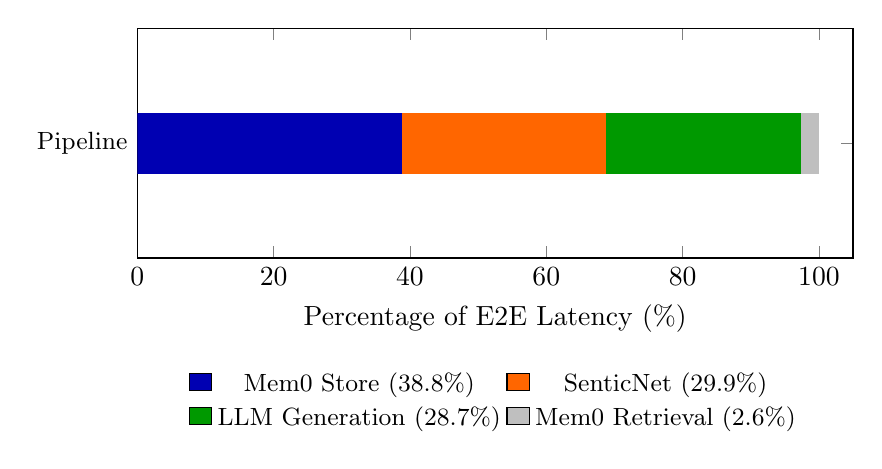
\begin{tikzpicture}
    \begin{axis}[
      xbar stacked,
      width=0.88\textwidth,
      height=4.5cm,
      bar width=22pt,
      xlabel={Percentage of E2E Latency (\%)},
      ytick={0},
      yticklabels={Pipeline},
      y tick label style={font=\small},
      xmin=0, xmax=105,
      xtick={0,20,40,60,80,100},
      legend style={
        at={(0.5,-0.45)},
        anchor=north,
        legend columns=2,
        font=\small,
        draw=none,
      },
      enlarge y limits=0.8,
    ]
      % Mem0 Store
      \addplot[fill=blue!70!black, draw=none] coordinates {(38.8,0)};
      % SenticNet
      \addplot[fill=orange!80!red, draw=none] coordinates {(29.9,0)};
      % LLM Generation
      \addplot[fill=green!60!black, draw=none] coordinates {(28.7,0)};
      % Mem0 Retrieval
      \addplot[fill=gray!50, draw=none] coordinates {(2.6,0)};

      \legend{Mem0 Store (38.8\%), SenticNet (29.9\%), LLM Generation (28.7\%), Mem0 Retrieval (2.6\%)}

      % Segment labels inside the bars
      \node[font=\scriptsize, text=white, anchor=center] at (axis cs:19.4,0) {38.8\%};
      \node[font=\scriptsize, text=white, anchor=center] at (axis cs:53.7,0) {29.9\%};
      \node[font=\scriptsize, text=white, anchor=center] at (axis cs:83.15,0) {28.7\%};
    \end{axis}
  \end{tikzpicture}
  \caption{Pipeline latency waterfall showing the percentage contribution of each component to the total end-to-end latency of 13,961~ms. Mem0 store dominates at 38.8\% and is amenable to asynchronous execution.}
  \label{fig:waterfall}
\end{figure}

% -----------------------------------------------------------------------------
\section{Energy Consumption}
\label{sec:energy-evaluation}

\subsection{Per-Component Energy Breakdown}
\label{subsec:energy-breakdown}

\Cref{tab:energy-breakdown} presents energy consumed per pipeline execution by hardware component. Total energy was 21,314~mJ (CV 2.8\%), dominated by the GPU at 71.8\% (15,298~mJ), followed by DRAM at 21.5\% (4,571~mJ) and CPU at 6.8\% (1,446~mJ). The ANE consumed no measurable energy, confirming that MLX routes all computation through the GPU for Qwen3-4B.

\begin{table}[htbp]
  \centering
  \caption{Energy consumption per pipeline execution by hardware component.}
  \label{tab:energy-breakdown}
  \begin{tabular}{@{}lrrc@{}}
    \toprule
    \textbf{Component} & \textbf{Energy (mJ)} & \textbf{\% Total} & \textbf{CV} \\
    \midrule
    GPU  & 15,298 & 71.8\% & 3.3\% \\
    DRAM &  4,571 & 21.5\% & 3.2\% \\
    CPU  &  1,446 &  6.8\% & 3.9\% \\
    ANE  &      0 &  0.0\% & ---   \\
    \midrule
    Total & 21,314 & 100\% & 2.8\% \\
    \bottomrule
  \end{tabular}
\end{table}

\subsection{Energy Distribution}
\label{subsec:energy-distribution}

\Cref{fig:energy-pie} visualises the energy distribution. The GPU concentration (71.8\%) suggests future optimisations should target GPU efficiency---e.g., 4-bit quantisation or ANE offloading of embedding and normalisation layers. DRAM energy (21.5\%) could be reduced through speculative decoding \cite{xu2024}.

% --- MERMAID BACKUP ---
% ```mermaid
% pie title Energy Breakdown per Inference
%   "GPU (71.8%)" : 71.8
%   "DRAM (21.5%)" : 21.5
%   "CPU (6.8%)" : 6.8
% ```
% --- END MERMAID ---

\begin{figure}[htbp]
  \centering
  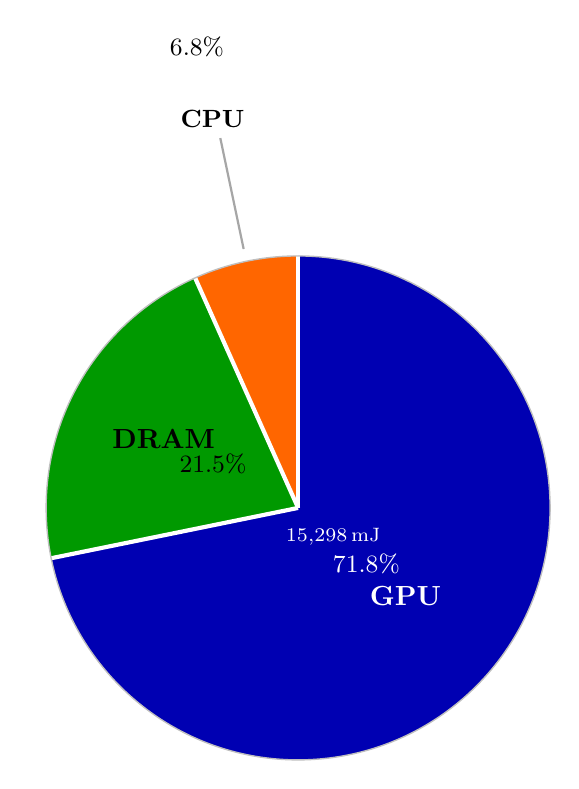
\begin{tikzpicture}
    % Angles: GPU = 71.8% of 360 = 258.48, DRAM = 21.5% of 360 = 77.4, CPU = 6.8% of 360 = 24.48
    \def\radius{3.2cm}

    % GPU slice: 0 to 258.48 degrees (blue)
    \fill[blue!70!black] (0,0) -- (90:\radius) arc (90:90-258.48:\radius) -- cycle;
    % DRAM slice: 258.48 to 335.88 degrees (green)
    \fill[green!60!black] (0,0) -- (90-258.48:\radius) arc (90-258.48:90-258.48-77.4:\radius) -- cycle;
    % CPU slice: 335.88 to 360 degrees (orange)
    \fill[orange!80!red] (0,0) -- (90-258.48-77.4:\radius) arc (90-258.48-77.4:90-360:\radius) -- cycle;

    % White divider lines
    \draw[white, line width=1.5pt] (0,0) -- (90:\radius);
    \draw[white, line width=1.5pt] (0,0) -- (90-258.48:\radius);
    \draw[white, line width=1.5pt] (0,0) -- (90-258.48-77.4:\radius);

    % Outer circle
    \draw[gray!50, line width=0.5pt] (0,0) circle (\radius);

    % GPU label (centroid of GPU arc)
    \node[font=\normalsize\bfseries, text=white] at (90-129.24:0.55*\radius) {GPU};
    \node[font=\small, text=white] at (90-129.24:0.35*\radius) {71.8\%};
    \node[font=\scriptsize, text=white] at (90-129.24:0.18*\radius) {15,298\,mJ};

    % DRAM label (centroid of DRAM arc)
    \pgfmathsetmacro{\drammid}{90-258.48-38.7}
    \node[font=\normalsize\bfseries] at (\drammid:0.6*\radius) {DRAM};
    \node[font=\small] at (\drammid:0.38*\radius) {21.5\%};

    % CPU label with callout (slice is small)
    \pgfmathsetmacro{\cpumid}{90-258.48-77.4-12.24}
    \draw[thick, gray!70] (\cpumid:1.05*\radius) -- (\cpumid:1.5*\radius);
    \node[font=\small\bfseries, anchor=north] at (\cpumid:1.65*\radius) {CPU};
    \node[font=\small, anchor=north] at (\cpumid:1.95*\radius) {6.8\%};
  \end{tikzpicture}
  \caption{Energy breakdown per pipeline execution by hardware component. GPU computation dominates at 71.8\%, reflecting the matrix multiplication-intensive nature of LLM inference on Apple Silicon.}
  \label{fig:energy-pie}
\end{figure}

\subsection{Battery Life Projections}
\label{subsec:battery-projections}

Idle power was 0.70~W (CPU~0.507~W, GPU~0.037~W, DRAM~0.157~W). \Cref{tab:battery-projections} projects battery life on a MacBook Pro M4 (72.4~Wh battery). Both scenarios comfortably exceed the 2\% per hour target from Objective~5, confirming negligible battery impact for sustained daily use.

\begin{table}[htbp]
  \centering
  \caption{Battery life projections under representative usage scenarios.}
  \label{tab:battery-projections}
  \begin{tabular}{@{}lcccc@{}}
    \toprule
    \textbf{Scenario} & \textbf{Inferences/hr} & \textbf{Energy/hr} & \textbf{Battery Life} & \textbf{Drain/hr} \\
    \midrule
    Active (1 msg/min)   & 60 & 3.74 Wh & $\sim$69 hr & $\sim$1.4\% \\
    Casual (1 msg/5 min) & 12 & 2.71 Wh & $\sim$96 hr & $\sim$1.0\% \\
    \bottomrule
  \end{tabular}
\end{table}

% -----------------------------------------------------------------------------
\section{Reproducibility Assessment}
\label{sec:reproducibility}

\Cref{tab:reproducibility-tiers} classifies all measured metrics into reproducibility tiers by CV. Core user-facing metrics---throughput (0.8\%), energy (2.8\%), and warm LLM latency (1.2\%)---fall in the ``Very High'' tier, while only cold start (33.8\%) and Mem0 retrieval (22.6\%) exhibit low reproducibility due to system-state sensitivity.

\begin{table}[htbp]
  \centering
  \caption{Reproducibility tier classification of evaluation metrics.}
  \label{tab:reproducibility-tiers}
  \begin{tabular}{@{}llp{7.5cm}@{}}
    \toprule
    \textbf{Tier} & \textbf{CV Range} & \textbf{Metrics} \\
    \midrule
    Deterministic & 0\%      & Classification coverage, Hourglass values, API reliability \\
    Very High     & $<$5\%   & Throughput (0.8\%), Energy (2.8\%), Warm LLM (1.2\%) \\
    High          & 5--15\%  & Generation time, SenticNet median (3\%) \\
    Moderate      & 15--25\% & Mem0 store (11.2\%), SenticNet mean (8.5\%) \\
    Low           & $>$25\%  & Cold start (33.8\%), Mem0 retrieval (22.6\%) \\
    \bottomrule
  \end{tabular}
\end{table}

% -----------------------------------------------------------------------------
\section{Evaluation Against Objectives}
\label{sec:objectives-evaluation}

\Cref{tab:traceability-matrix} presents the traceability matrix mapping each project objective to its evaluation criterion, measured result, and achievement status. All five objectives were met or exceeded.

Objective~1 (on-device LLM coaching) was achieved with 37.1 tok/s and 1.4--2.7~s warm latency, exceeding the 30 tok/s target by 23.7\% and aligning with edge deployment benchmarks for 3--7B parameter models on Apple Silicon \cite{lin2025, xu2024}. Objective~2 (emotion classification $\geq$80\%) was exceeded at 86\% accuracy with only 210 training sentences, demonstrating that contrastive learning extracts sufficient signal from fewer than 35 sentences per category \cite{reimers2019, cambria2016}. Objective~3 (SenticNet integration) achieved 100\% API reliability with deterministic Hourglass values, consistent with neurosymbolic AI design principles \cite{cambria2024}. Objective~4 (screen classification and JITAI) achieved 549 titles/s with 78\% rule-based coverage and seven intervention rules (including four emotion-aware rules driven by confidence-gated SetFit predictions), all verified by 20~dedicated wiring tests. Objective~5 (resource efficiency) achieved 21,314~mJ per execution ($\sim$1.4\%/hr drain) and $<$3~GB RSS---a 2$\times$ margin on the 6~GB target---validating on-device deployment viability \cite{hannun2023}.

\begin{table}[htbp]
  \centering
  \caption{Objective-to-result traceability matrix.}
  \label{tab:traceability-matrix}
  \begin{tabular}{@{}p{2.8cm}p{3.2cm}p{4.5cm}l@{}}
    \toprule
    \textbf{Objective} & \textbf{Criterion} & \textbf{Result} & \textbf{Status} \\
    \midrule
    Obj 1: On-device LLM & Interactive speed & 37.1 tok/s, 1.4--2.7\,s latency & Achieved \\[4pt]
    Obj 2: Emotion classification & $\geq$80\% accuracy & 86\%, 0.862 macro-F1 & Exceeded (1.08$\times$) \\[4pt]
    Obj 3: SenticNet + CBM & Reliable, meaningful & 100\% reliability, stdev 48--67 & Achieved \\[4pt]
    Obj 4: Screen + JITAI & Real-time classification & 549 titles/s, 7 rules (4 emotion), 20 wiring tests & Exceeded \\[4pt]
    Obj 5: Resource efficiency & Minimal battery, $<$6\,GB & 21,314\,mJ, $<$3\,GB, $\sim$1.4\%/hr & Exceeded (2$\times$ margin) \\
    \bottomrule
  \end{tabular}
\end{table}

\subsection{Summary of Findings}
\label{subsec:evaluation-summary}

The evaluation demonstrates that the ADHD Second Brain achieves all five project objectives, with three exceeded by substantial margins. Two architectural trade-offs warrant acknowledgement: the SenticNet cloud API dependency means 68.7\% of end-to-end latency originates from network calls, creating tension between privacy goals and ontology freshness; and the 51.7\% affective computing overhead represents the quantitative cost of emotion-aware coaching---a trade-off accepted for its clinical value in ADHD support \cite{beattie2025, faraone2021}.
